\section{Part 2}
A quick and simple way to implement a BAD algorithm is to measure the power from the input signal.
Mathematically described, the power equation is given by the following formula: 
\[
P(n) = \frac{1}{N} \sum\limits_{k=0}^{N-1} x^2(n-k)
\]
where $P(n)$ is a vector. Since the BAD application is calculating the power of the input signal in 
real-time, this equation becomes impossible to implement. Hence, the usage of the \emph{recursive
averaging} algorithm. It is, in perspective of memory usage, a light and hardware friendly algorithm 
that calculates the average power level of the signal. Given below,
\[
P(n) = \alpha P(n-1)+(1-\alpha)x^2(n)
\]
instead of performing the calculation for one sample at the time, a block of the samples are calculated and summed.
The old result is saved to be used as $P(n-1)$. The $\alpha$ is a constant between 0 and 1 and is related to the 
time by the following formula:
\[
\alpha = \frac{1}{T_{s}F_{s}}
\]
By having two different $\alpha$ values, when the power is increasing respective decreasing, the algorithm
can response faster and the decrease slower. That way, hard spikes are avoided and the average power is slowly
fading,causing quicker reacting if high power signals enter the system.

The advanced algorithm is based upon the on the same, \emph{recursive averaging}, algorithm.
In addition, a filter is added to remove the noise which should increase the precision for the wanted interval (explained below).

Three various baby and noise sounds were provided. The sample frequency for all of the recorded 
files are 8 kHz. In Figure \ref{fig:baby_spec} and Figure \ref{fig:noise_spec} the power/frequency 
spectrum is plotted for baby respective noise sounds. Because the power level is unproportionally 
low for some baby sound recordings an enhanced plot is displayed in Figure~\ref{fig:enhanced}. 
From the plots it can be seen that the baby sound spectrum is between $\sim$ 300-2500 Hz and the 
noise sound spectrum is below 200 Hz and between $\sim$1300-2100 Hz. To get the wanted effect from 
the advanced algorithm a bandpass filter with a window between 300-1300 Hz is the optimal solution. 
The noise is filtered but the baby sound are kept.

\begin{figure}[h]
  \centering
  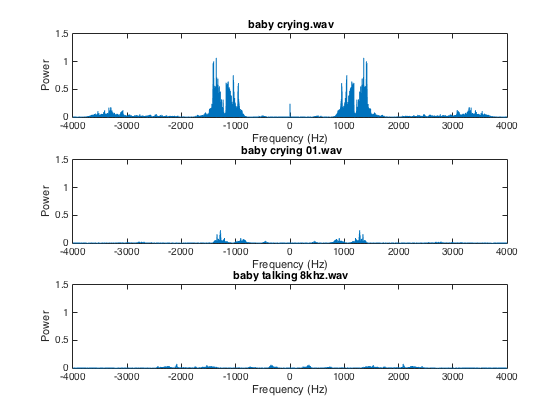
\includegraphics[width=1\textwidth]{sections/freq_spec_baby_linkaxis.png}
  \caption{Bla bla bla}
  \label{fig:baby_spec}
\end{figure}

\begin{figure}[h]
  \centering
  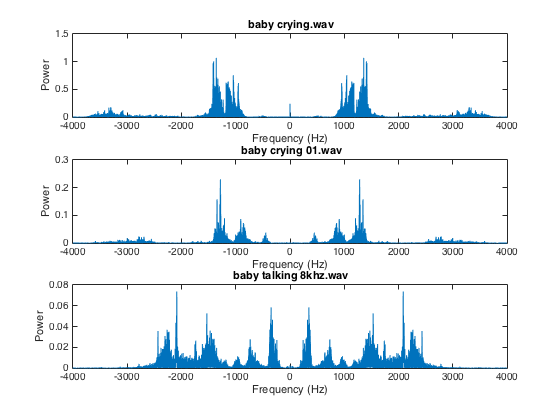
\includegraphics[width=1\textwidth]{sections/freq_spec_babyFix.png}
  \caption{Bla bla bla}
  \label{fig:enhanced}
\end{figure}

%\begin{figure}[!hp]
%  \centering
%  \begin{minipage}[b]{0.4\textwidth}
%    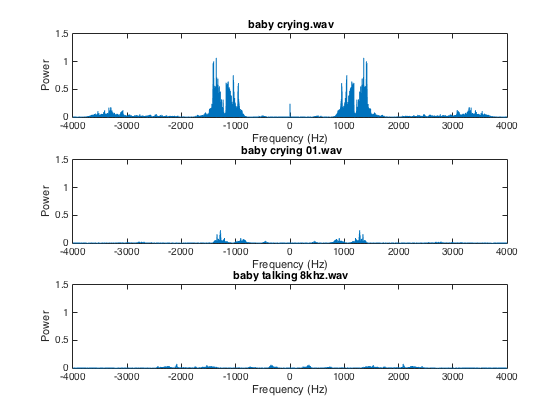
\includegraphics[width=1\textwidth]{sections/freq_spec_baby_linkaxis.png}
%    \caption{Fig111}
%  \end{minipage}
%  \hfill
%  \begin{minipage}[b]{0.4\textwidth}
%    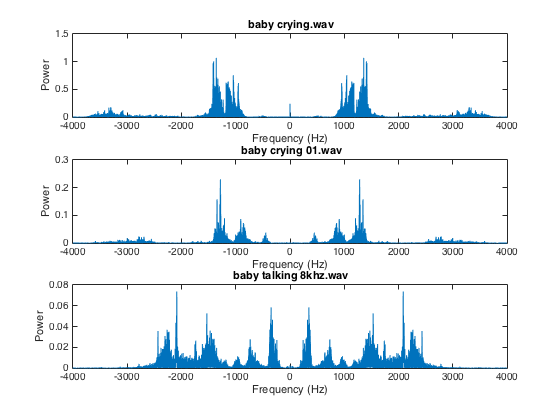
\includegraphics[width=1\textwidth]{sections/freq_spec_babyFix.png}
%    \caption{Fig222}
%  \end{minipage}
%\end{figure}

\begin{figure}
  \centering
  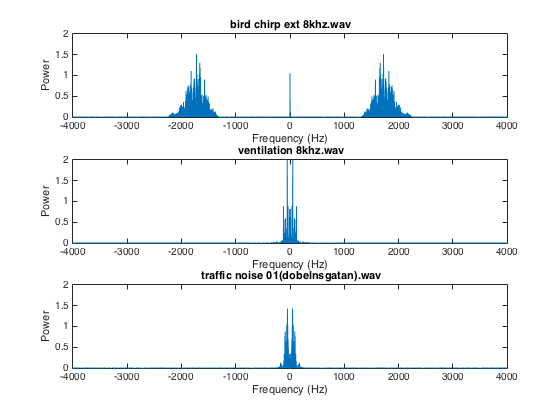
\includegraphics[width=1\textwidth]{sections/freq_spec_noise_linkaxis.png}
  \caption{Bla bla bla}
  \label{fig:noise_spec}
\end{figure}
